\documentclass{article}%
\usepackage[T1]{fontenc}%
\usepackage[utf8]{inputenc}%
\usepackage{lmodern}%
\usepackage{textcomp}%
\usepackage{lastpage}%
\usepackage[head=40pt,margin=0.5in,bottom=0.6in]{geometry}%
\usepackage{graphicx}%
%
\title{\textbf{Federación de Trabajadores públicos rechaza ir a paralizaciones}}%
\author{Diario El Universal}%
\date{07/03/2019}%
%
\begin{document}%
\normalsize%
\maketitle%
\textbf{URL: }%
http://www.eluniversal.com/politica/34965/federacion{-}de{-}trabajadores{-}publicos{-}rechazan{-}ir{-}a{-}paralizaciones\newline%
%
\textbf{Periodico: }%
EU, %
ID: %
34965, %
Seccion: %
politica\newline%
%
\textbf{Palabras Claves: }%
NO\_TIENE\newline%
%
\textbf{Derecho: }%
2.1%
, Otros Derechos: %
\newline%
%
\textbf{\textit{El presidente de la Federación Nacional de Trabajadores del Sector Público (Fentrasep), Franklin Rondón informó que se estarán conformando "Los Comandos de Defensas de las Instituciones Públicas"}}%
\newline%
\newline%
%
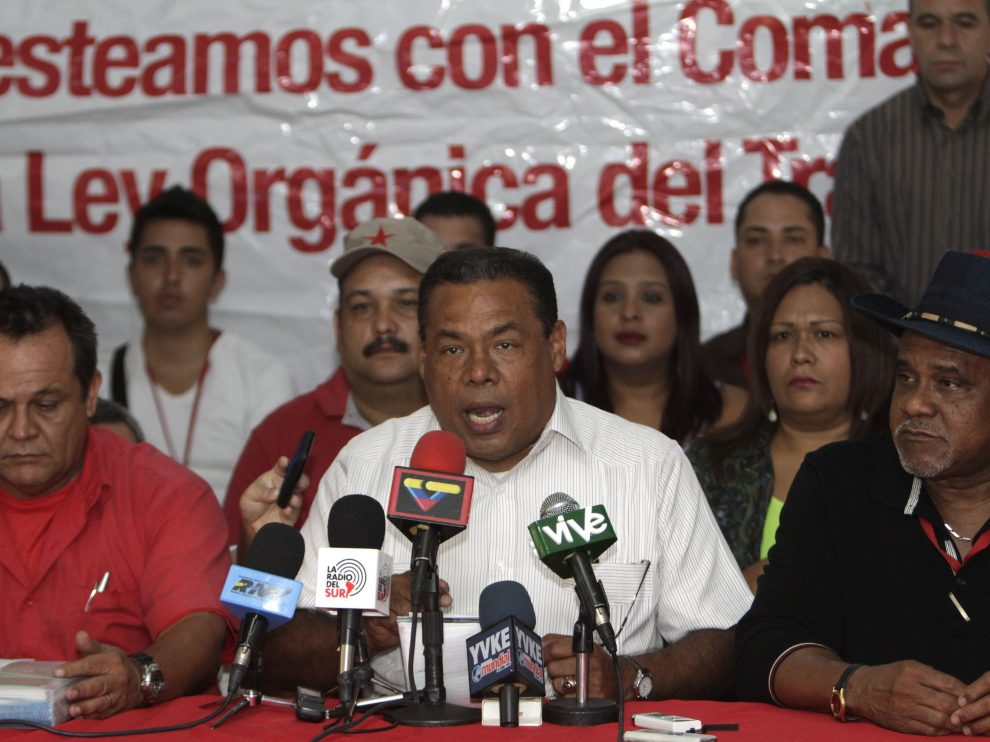
\includegraphics[width=300px]{EU_34965.jpg}%
\newline%
%
El presidente de la Federación Nacional de Trabajadores del Sector Público (Fentrasep), Franklin Rondón, expresó este miércoles el rechazo de la agrupación que representa al anuncio del diputado Juan Guaidó, de promover "paros escalonados" entre los trabajadores de la administración pública.%
\newline%
%
Ayer, después de una larga reunión en la sede del Metro de Caracas, en La Hoyada, Rondón desconoció a Guaidó como "presidente encargado" y a su vez anunció que representantes de las distintas áreas de la administración pública rechazan el llamado a paro y que  presentes en el encuentro, decidieron, muy contrariamente al llamado a Guaidó, en primer lugar, llamar a la unidad del sector laboral para hacer frente a las amenazas de la oposición; constituirse en cada sindicato en "comandos" en defensa del funcionamiento de las distintas dependencias gubernamentales, con el fin de garantizar el mejor funcionamiento de los servicios que en ellos se presten; y, en tercer lugar, advertir que "si tumban a Maduro, si van a ver una verdadera huelga", porque, según sostuvo, el grupo de la oposición que encabeza Guaidó "no representa a la clase trabajadora" del país.%
\newline%
%
El pasado lunes, dirigentes laborales del sector público se reunieron con Guaidó, quien anunció a que a  petición de los propios trabajadores se daría inicio a una serie de paros en esa área.%
\newline%
%
\end{document}